\StartPlate{V32}{The current frontier}{Completed finite and restricted work remains reusable without relabeling the open endpoints.}
\begin{center}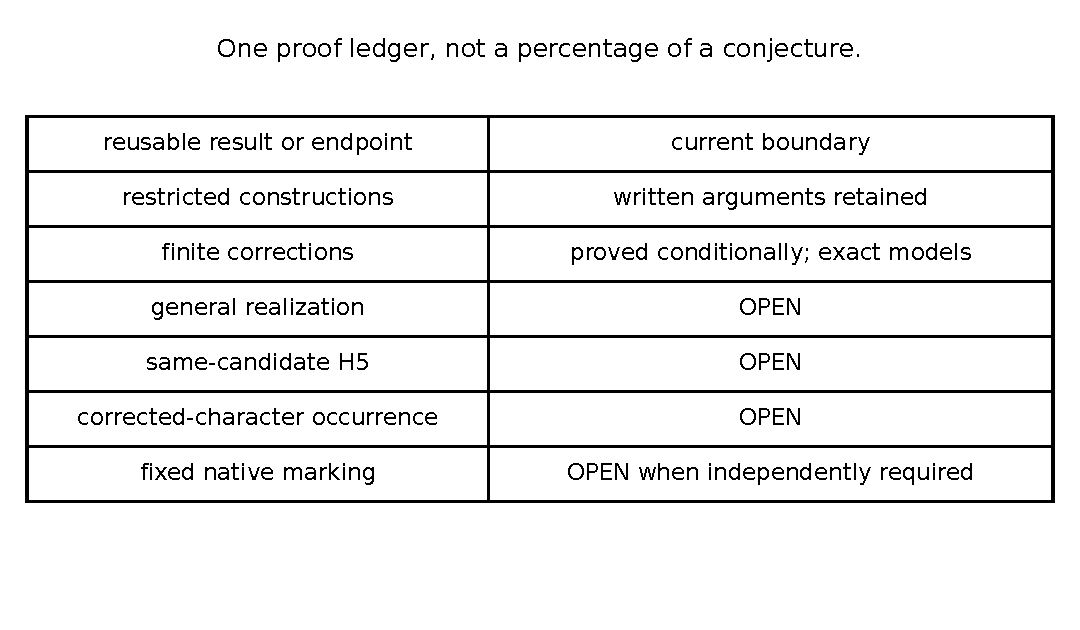
\includegraphics[width=\linewidth]{figures/V32.pdf}\end{center}
The progress record now has a distinct visual reading route through the restricted constructors, finite comparison mechanisms, exact obstructions, and conditional corrections. These are substantive results and reusable arguments. Their existence does not make the remaining arithmetic statements interchangeable.

General realization requires an actual common host with the admitted actions and transports. Same-candidate H5 requires the characterizing factors for that very realizer. The corrected-character problem requires occurrence in the original specified induction candidate. An independently fixed native marking, when required, needs the actual certificate on V30.

This atlas is Publication Block 5. It leaves the 77-page research paper byte-preserved at v0.4.0. The original 109-page monograph, 51-page visual guide, and 234-page Lean guide are inherited baselines awaiting coordinated revision. No fresh Lean compilation or external peer review is claimed. The versioned ledger records these separate statuses and the exact next editorial step rather than assigning a conjecture-completion percentage.
\vfill\PlateSource{Versioned claim map}{Part I, Section 12; Part II, Section 20; Part III, Section 30}{29}
